\documentclass[UTF8,zihao=-4]{ctexart}
\usepackage[a4paper,margin=2.5cm]{geometry}
\usepackage{amsmath, amssymb, amsthm}
\usepackage{bm}
\usepackage{hyperref}
\usepackage{graphicx}
\usepackage{caption}
\usepackage{listings}
\usepackage{xcolor}
\usepackage{float}
\usepackage{placeins}
\graphicspath{{figures/}}

% Code style
\lstdefinestyle{code}{
  basicstyle=\ttfamily\small,
  numbers=left,
  numberstyle=\tiny,
  numbersep=8pt,
  keywordstyle=\color{blue},
  commentstyle=\color{teal!70!black},
  stringstyle=\color{orange!70!black},
  showstringspaces=false,
  breaklines=true,
  frame=single,
  framerule=0.3pt,
  rulecolor=\color{black!15}
}
\lstset{style=code}

\title{多模态基础模型与大模型高效微调}
\author{}
\date{\today}

\begin{document}
\maketitle
\tableofcontents
\FloatBarrier

\section{CLIP、Flamingo、GPT-4、LLaVA}
多模态基础模型通过跨模态对齐学习统一表征,支持零样本识别、图像条件生成与交互式推理。图~\ref{fig:clip_multimodal_alignment_cn} 对比了代表性架构的嵌入空间。

\subsection{对比式语言-图像预训练(CLIP)}
CLIP 由图像编码器 $f_{\theta}$ 与文本编码器 $g_{\phi}$ 组成,在 4 亿图文对上进行对比学习。对 batch 大小 $B$,图像嵌入 $\mathbf{v}_i = f_{\theta}(\mathbf{x}_i)$,文本嵌入 $\mathbf{t}_i = g_{\phi}(\mathbf{y}_i)$ 均做归一化,通过双向交叉熵优化:
\begin{align}
  \ell_{\text{img}} &= -\frac{1}{B} \sum_{i=1}^{B} \log \frac{\exp(\mathbf{v}_i^\top \mathbf{t}_i / \tau)}{\sum_{j=1}^{B} \exp(\mathbf{v}_i^\top \mathbf{t}_j / \tau)}, \\
  \ell_{\text{text}} &= -\frac{1}{B} \sum_{i=1}^{B} \log \frac{\exp(\mathbf{t}_i^\top \mathbf{v}_i / \tau)}{\sum_{j=1}^{B} \exp(\mathbf{t}_i^\top \mathbf{v}_j / \tau)}, \\
  \mathcal{L}_{\text{CLIP}} &= \tfrac{1}{2} (\ell_{\text{img}} + \ell_{\text{text}}).
\end{align}
学习到的温度 $\tau$ 控制相似度的锐度。零样本分类通过提示工程替代分类头:$\hat{y} = \arg\max_{k} \mathbf{v}_{\mathrm{test}}^\top \mathbf{t}_k$,其中 $\mathbf{t}_k$ 对应 ``a photo of a \{label\}'' 的提示句嵌入。

\subsection{Flamingo:基于 Perceiver 的视觉语言模型}
Flamingo 将冻结的视觉编码器与语言模型通过门控交叉注意力(Gated XAttn-Dense)层耦合。文本隐藏状态 $\mathbf{h}_{\mathrm{LM}}$ 与视觉特征 $\mathbf{h}_{\mathrm{vis}}$ 的交互为:
\begin{align}
  \mathbf{z} &= \mathrm{MultiHeadQK}(\mathbf{h}_{\mathrm{LM}}, \mathbf{h}_{\mathrm{vis}}), \\
  \mathbf{m} &= \sigma(\mathbf{W}_g [\mathbf{h}_{\mathrm{LM}}, \mathbf{z}]) \odot \mathbf{W}_m \mathbf{z}, \\
  \mathbf{h}'_{\mathrm{LM}} &= \mathbf{h}_{\mathrm{LM}} + \mathbf{m}.
\end{align}
Perceiver Resampler 将任意长度的视觉 token 压缩为固定长度潜变量,使 Flamingo 在少样本多模态任务上具备快速适应能力。

\subsection{GPT-4 多模态扩展}
公开信息显示,GPT-4 通过视觉编码器与投影层将图像 patch 嵌入对齐到语言模型隐层维度,结合联合位置编码,实现文本与视觉 token 的交替输入;并采用多模态 RLHF 对对话输出进行强化。模型擅长解析图表、流程图等复合信息,是通用助手的重要里程碑。

\subsection{LLaVA:大语言+视觉助手}
LLaVA 将 CLIP 视觉编码器与 Vicuna 语言模型结合,通过投影矩阵 $W_{\text{proj}}$ 将视觉特征 $\mathbf{v}$ 映射到语言维度 $d$:
\begin{equation}
  \tilde{\mathbf{v}} = W_{\text{proj}} \mathbf{v}, \quad \mathbf{H}_0 = [\text{BOS}, \tilde{\mathbf{v}}, \text{文本 token}].
\end{equation}
训练流程分两阶段:
\begin{enumerate}
  \item \textbf{视觉指令微调:} 使用 GPT 生成的图文对话执行监督微调。
  \item \textbf{对齐优化:} 采用偏好优化(如 DPO)提高回答质量与兼容性。
\end{enumerate}
在 ScienceQA、VizWiz 等基准上取得优异结果。

\begin{figure}[H]
  \centering
  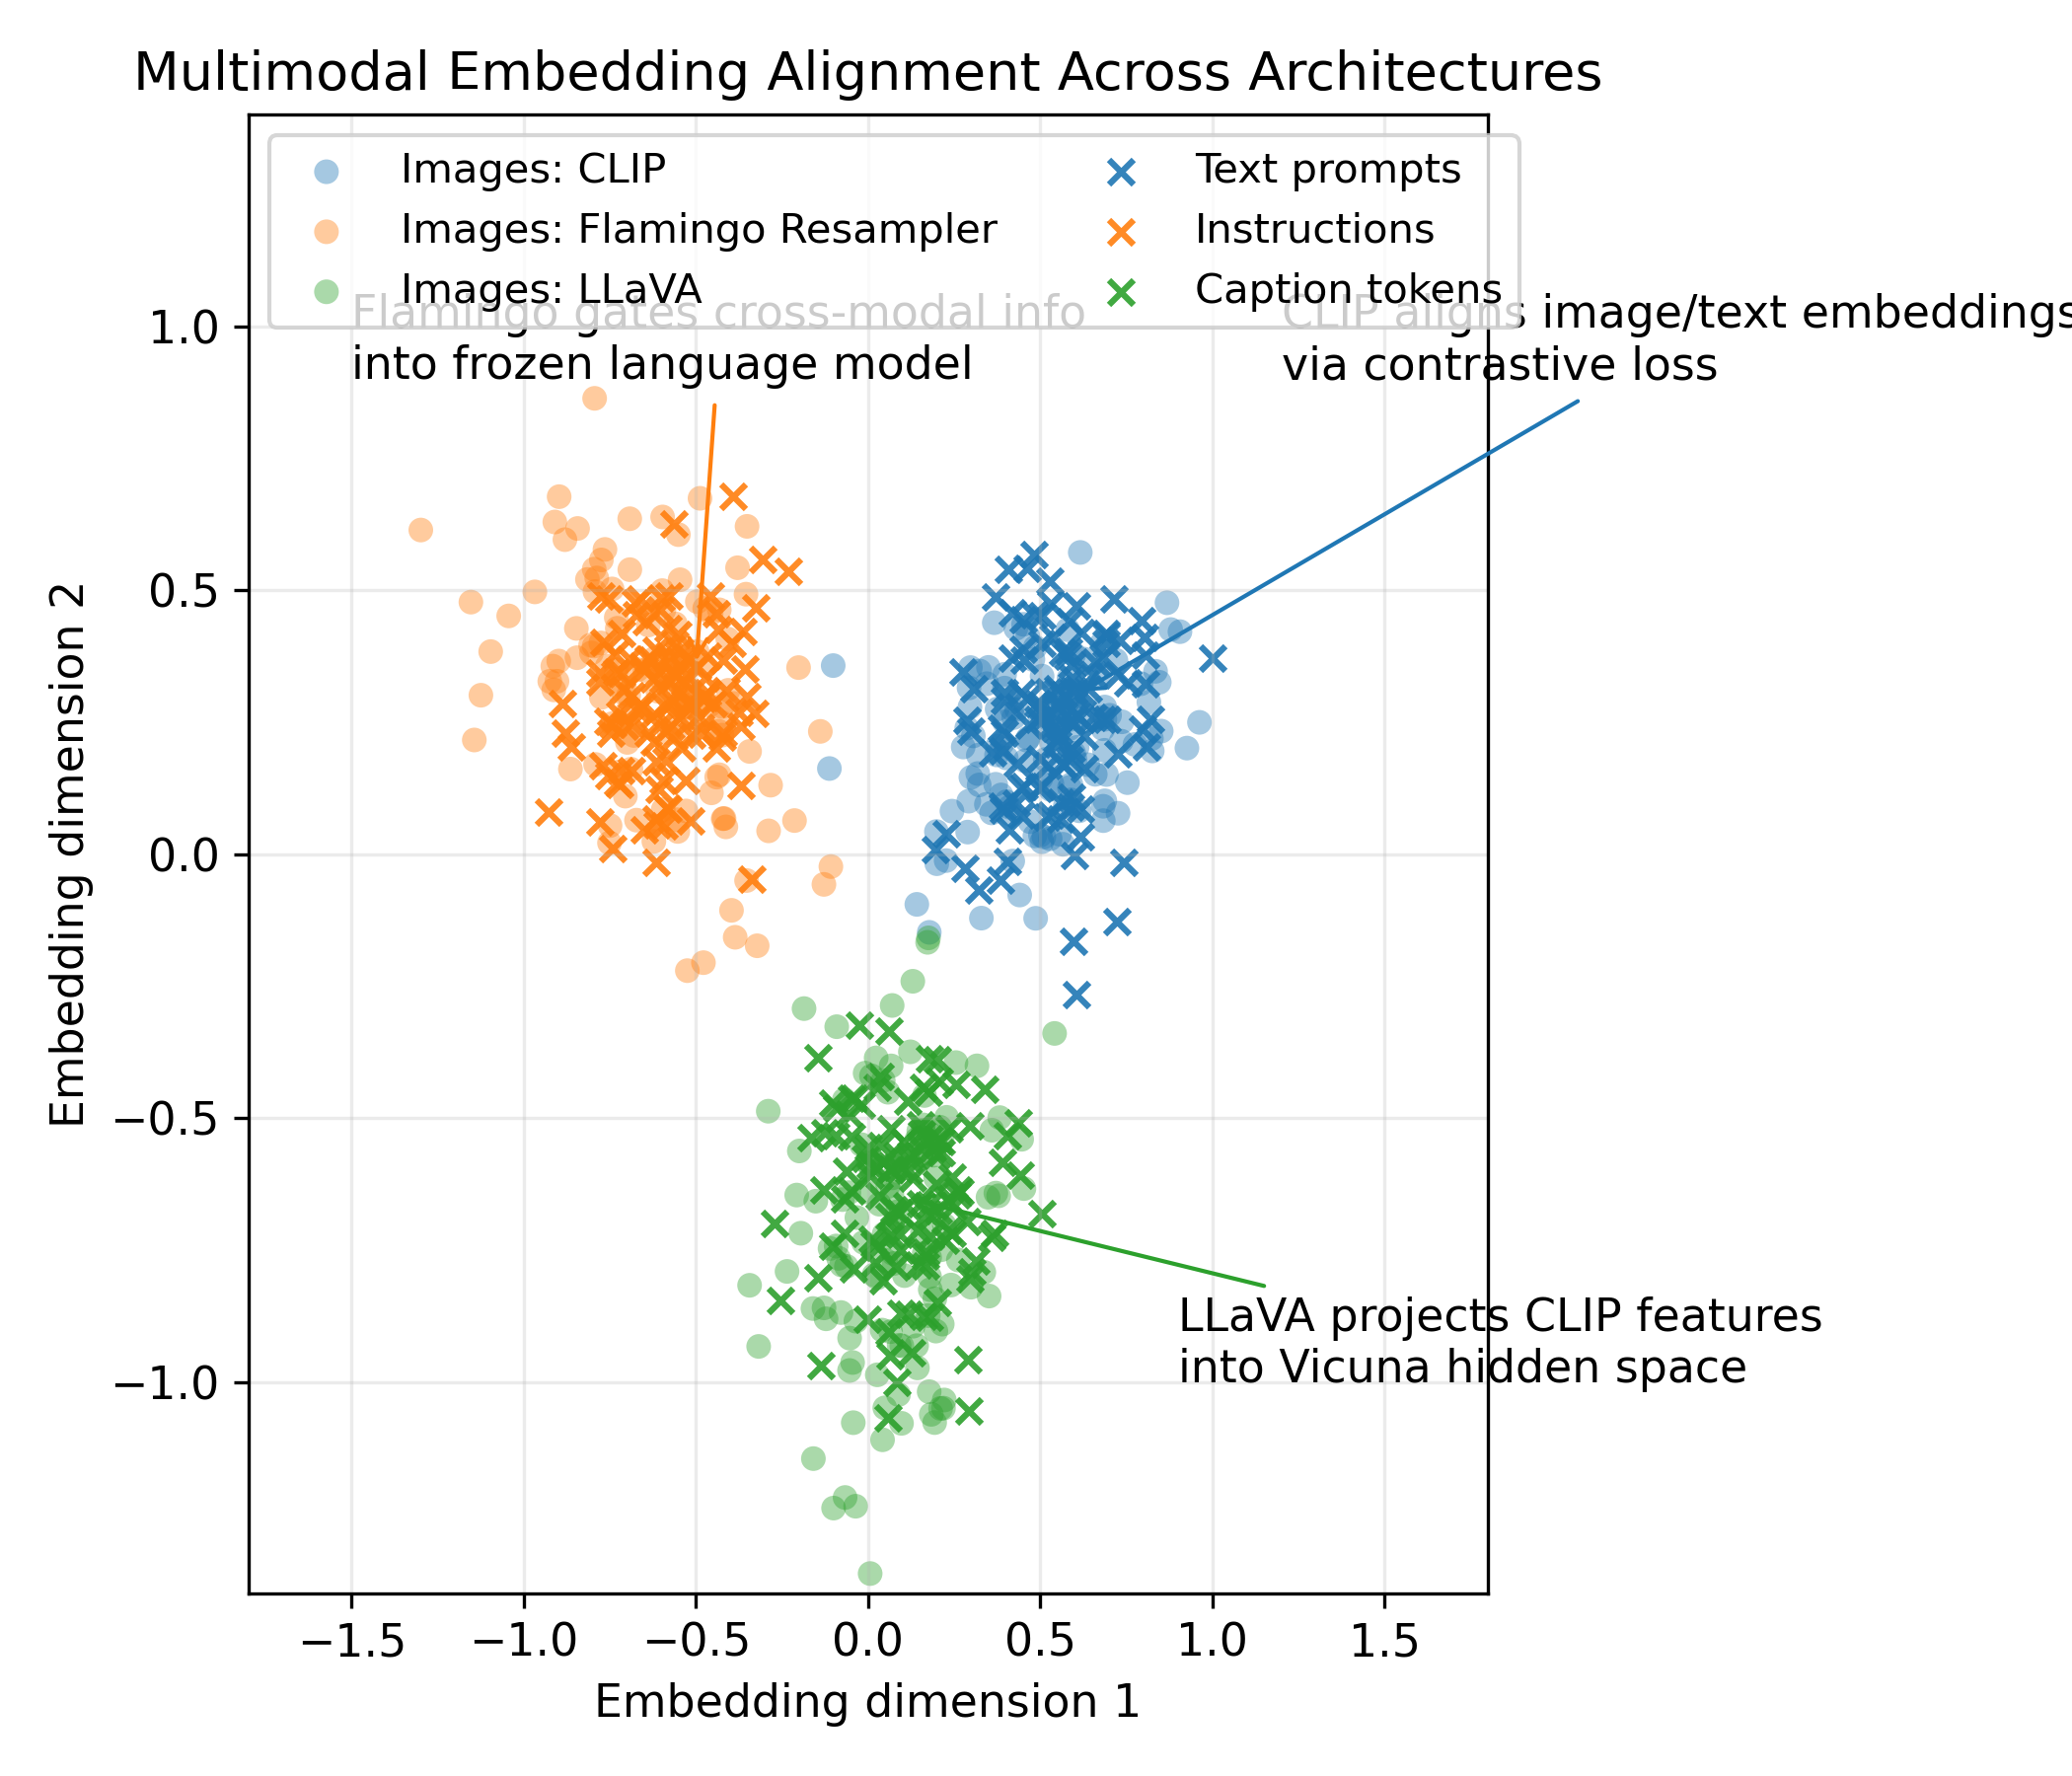
\includegraphics[width=0.85\textwidth]{clip_multimodal_alignment.png}
  \caption{CLIP、Flamingo、GPT-4 与 LLaVA 的嵌入对齐示意。CLIP 学得统一空间,而 Flamingo、LLaVA 通过桥接层连接视觉与语言模型。}
  \label{fig:clip_multimodal_alignment_cn}
\end{figure}
\FloatBarrier

\section{大模型的训练与微调:LoRA、PEFT、RAG}
大规模模型的全量微调成本高昂,参数高效微调(PEFT)通过插入轻量模块实现快速适配;检索增强生成(RAG)则利用外部知识降低幻觉。图~\ref{fig:lora_rank_update_cn} 与图~\ref{fig:rag_pipeline_cn} 展示了核心机制。

\subsection{低秩适配(LoRA)}
LoRA 冻结原权重 $\mathbf{W}_0$,只训练低秩更新 $\Delta \mathbf{W} = \mathbf{B} \mathbf{A}$(秩 $r \ll d$):
\begin{equation}
  \mathbf{W} = \mathbf{W}_0 + \frac{\alpha}{r} \mathbf{B} \mathbf{A}, \quad \mathbf{A} \in \mathbb{R}^{r \times d_{\text{in}}}, \; \mathbf{B} \in \mathbb{R}^{d_{\text{out}} \times r}.
\end{equation}
对隐藏向量 $\mathbf{h}$ 的前向计算:
\begin{equation}
  \mathbf{y} = \mathbf{W}_0 \mathbf{h} + \frac{\alpha}{r} \mathbf{B} (\mathbf{A} \mathbf{h}).
\end{equation}
仅训练 $\mathbf{A}, \mathbf{B}$,参数量降至 $\mathcal{O}(r(d_{\text{in}} + d_{\text{out}}))$。常用秩为 4/8/16,需在容量与存储间折衷。

\subsection{前缀/提示微调与 AdapterFusion}
PEFT 包含多种策略:
\begin{itemize}
  \item \textbf{前缀微调:} 为每层注意力的键/值矩阵学习虚拟 token。
  \item \textbf{提示微调:} 只在输入层优化连续提示嵌入。
  \item \textbf{适配器:} 插入带残差的瓶颈 MLP。AdapterFusion 可在多个任务适配器上学习加权组合,实现迁移复用。
\end{itemize}
Hugging Face PEFT 等库为这些方法提供统一接口,可组合应用(如 LoRA + Prompt Tuning)。

\subsection{检索增强生成(RAG)}
RAG 通过检索文档 $\{\mathbf{d}_k\}_{k=1}^{K}$ 为查询 $\mathbf{q}$ 提供知识支撑:
\begin{equation}
  \mathbf{d}_k = \mathrm{Retrieve}(\mathbf{q}, \mathcal{D}), \qquad \mathbf{y} \sim p_{\theta}(\mathbf{y} \mid \mathbf{q}, \mathbf{d}_{1:K}).
\end{equation}
密集检索器(DPR、Contriever)使用双塔编码器训练对比损失。生成阶段常见方式:
\begin{itemize}
  \item \textbf{FiD:} 将每个检索段的编码输出拼接后送入解码器交叉注意力。
  \item \textbf{RAG-token / RAG-sequence:} 在自回归解码过程中对检索文档求边缘化。
\end{itemize}
生产部署需考虑检索索引的定期更新以及缓存策略以降低延迟。

\subsection{实现示例}
\begin{lstlisting}[language=Python, caption={基于 Hugging Face PEFT 的 LoRA + RAG 组合示例。}]
from peft import LoraConfig, get_peft_model
from transformers import AutoModelForCausalLM, AutoTokenizer
from rag_pipeline import DenseRetriever, format_context

base_model = AutoModelForCausalLM.from_pretrained("meta-llama/Llama-2-7b-hf", device_map="auto")
tokenizer = AutoTokenizer.from_pretrained("meta-llama/Llama-2-7b-hf")

lora_config = LoraConfig(
    r=8,
    lora_alpha=32,
    lora_dropout=0.1,
    target_modules=["q_proj", "v_proj"],
)
model = get_peft_model(base_model, lora_config)

retriever = DenseRetriever(index_path="faiss.index")

def generate_with_rag(question: str):
    docs = retriever.search(question, top_k=5)
    prompt = format_context(question, docs)
    inputs = tokenizer(prompt, return_tensors="pt").to(model.device)
    outputs = model.generate(**inputs, max_new_tokens=256, temperature=0.7)
    return tokenizer.decode(outputs[0], skip_special_tokens=True)
\end{lstlisting}

\subsection{工程考量}
\begin{itemize}
  \item \textbf{内存占用:} LoRA 权重单独存储(几十 MB 级),便于快速切换任务。
  \item \textbf{评价体系:} 需结合人类偏好测试,Rouge/BLEU 等离线指标不足以刻画对话质量。
  \item \textbf{安全合规:} 检索过滤与响应审核可减少敏感信息泄露。
\end{itemize}

\begin{figure}[H]
  \centering
  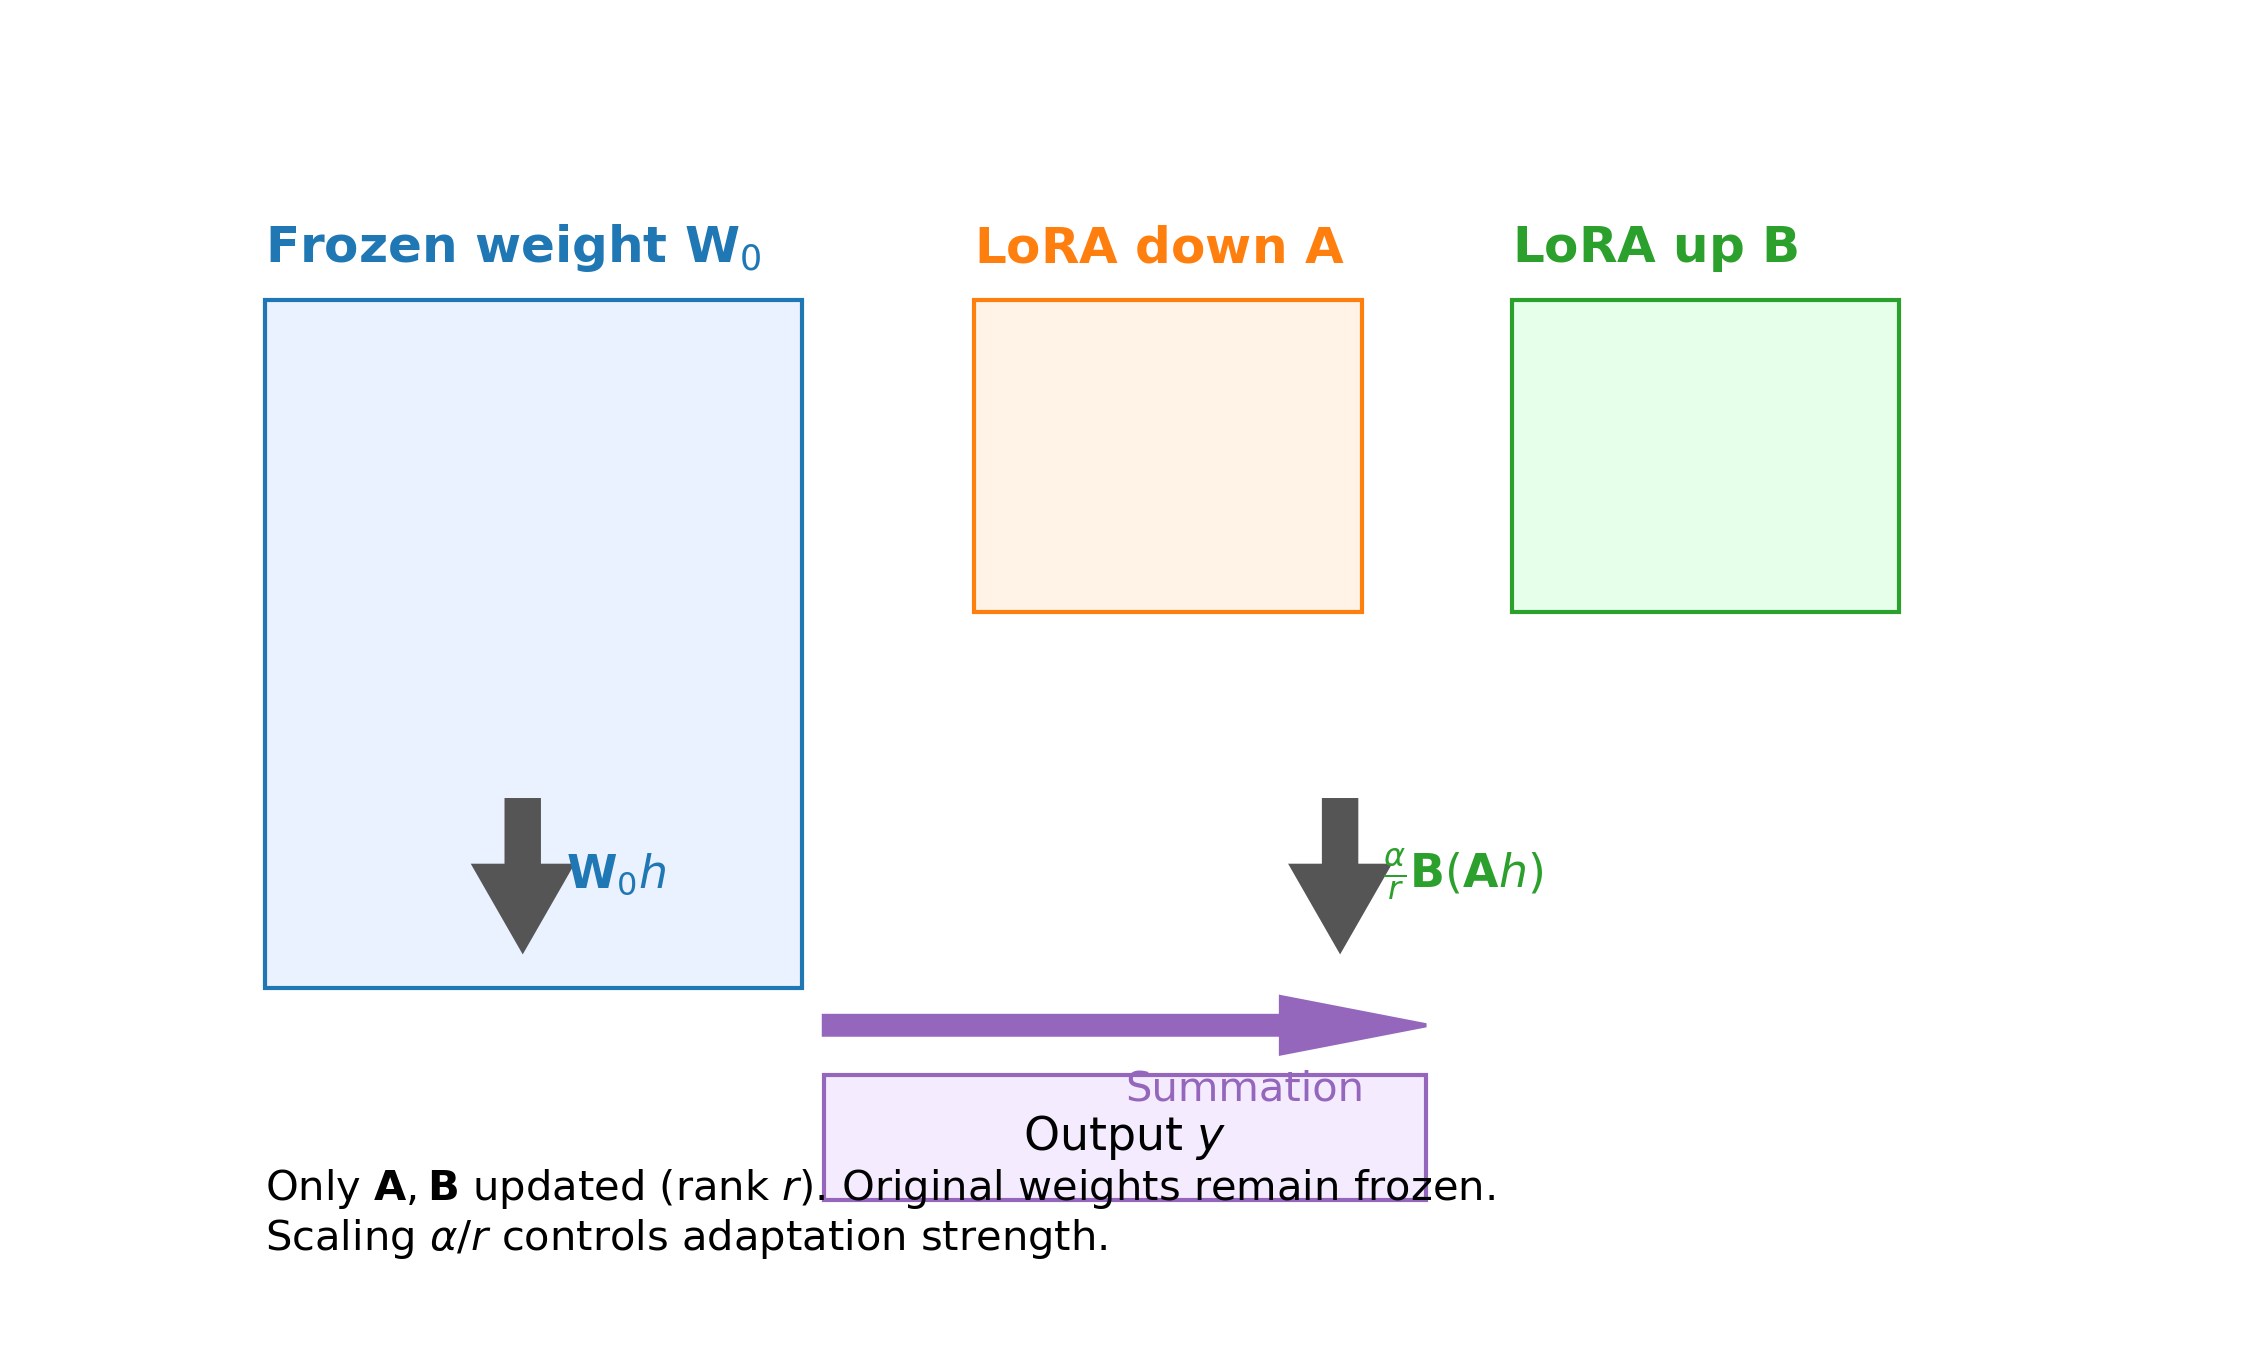
\includegraphics[width=0.85\textwidth]{lora_rank_update.png}
  \caption{LoRA 在注意力投影中插入低秩适配器,秩与缩放控制表达能力。}
  \label{fig:lora_rank_update_cn}
\end{figure}

\begin{figure}[H]
  \centering
  
\includegraphics[width=0.9\textwidth]{rag_pipeline.png}
  \caption{检索增强生成流程:查询编码、文档检索、上下文融合与响应生成。}
  \label{fig:rag_pipeline_cn}
\end{figure}
\FloatBarrier

\section*{延伸阅读}
\begin{itemize}
  \item Alec Radford 等:《Learning Transferable Visual Models From Natural Language Supervision》,ICML 2021。
  \item Jean-Baptiste Alayrac 等:《Flamingo: A Visual Language Model for Few-Shot Learning》,NeurIPS 2022。
  \item OpenAI:《GPT-4 Technical Report》,2023。
  \item Hu 等:《LoRA: Low-Rank Adaptation of Large Language Models》,ICLR 2022。
  \item Lewis 等:《Retrieval-Augmented Generation for Knowledge-Intensive NLP Tasks》,NeurIPS 2020。
\end{itemize}

\end{document}
